\documentclass{article}
\usepackage{graphicx}
\usepackage{minted}
\usepackage{ngerman}
\usepackage{geometry}
\graphicspath{ {./images/} }
\title{AvailabilityMatrix}
\author{Johannes Karrer \& Elias Walder}

\geometry{
	top=2cm,
	bottom=2.5cm,
	left=3.0cm,
	right=3.0cm,
}


\begin{document}
	\maketitle
	\section{Problem}
	Es wird eine geeignete Datenstruktur benötigt, um die verfügbaren Zeiten der einzelnen Räume abzubilden und gleichzeitig das Eintragen von CourseSessions zu ermöglichen.
	
	Die Datenstruktur muss darüber hinaus effizient auf verschieden Constraints überprüft werden können, unter anderem:
	
	\begin{itemize}
		\item Kurse desselben Semsters dürfen nicht am gleichen Tag zur gleichen Zeit stattfinden, damit sie sich für die Studierenden des jeweiligen Semsters nicht überschneiden.
		\item Kurse, die zeitlich aufgeteilt wurden (z. B. eine 3-stündige Vorlesung in 2 und 1 Stunde), sollten nicht am gleichen Tag stattfinden.
		\item Kurse mit mehreren Gruppen (PS) sollten nicht alle zur selben Zeit stattfinden, damit die Einteilung für Studierende flexibler möglich ist.
	\end{itemize}
	
	\section{Lösungsansatz: AvailabilityMatrix}
	
	
	Eigenschaften:
	\begin{itemize}
		\item $n \times 5$ Matrix
		\begin{itemize}
			\item Jede Spalte repräsentiert dabei einen Wochentag (S1: MON, S2: DIE, ...)
			\item Jede Zeile repräsentiert 15 Minuten des Tages (Z1: [t0,t0+15), Z2: [t0+15,t0+30), ...)
			\item Jeder Eintrag in der AvailabilityMatrix eines Raumes ist eine Referenz auf die\\ CourseSession, die diesem Raum zu einer bestimmten Zeit zugeordnet ist.\\
			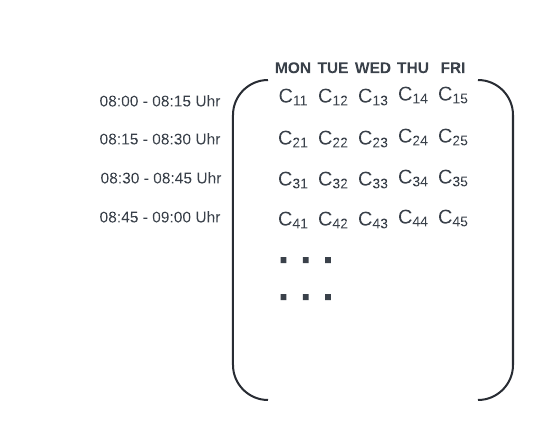
\includegraphics{AvailabilityMatrix}
		\end{itemize}
		\item Vorteile:
		\begin{itemize}
			\item Durch die 15-Minuten-Intervalle lassen sich Kurse unterschiedlicher Länge gut darstellen.
			\item Die Darstellung der Matrix ist sehr intuitiv und ähnelt der Darstellung eines Wochenkalenders
			\item Der Ansatz ist flexibel und für unsere Anforderungen auch gut skalierbar.
		\end{itemize}
	\end{itemize}
	
	
	
	
	
	
	
	
	
	
	
	
	
	
	
	
	
	
	
	
	
	
	
	
	
	
	
	
\end{document}
